\chapter{Алгоритмы генерации и обработки данных} \label{chapt2}

В этой главе описываются постановки задач аппроксимации данных, а также исследованные алгоритмы генерации 
синтетических данных и
экстраполяции тарировочных данных. 


\section{Подходы к аппроксимации функций}\label{sect2_1}
% поправить слова
Метод наименьших квадратов --- один из базовых методов для оценки неизвестных 
параметров моделей по набору данных, при этом исследуется на минимум
следующая функция

\begin{equation}
\label{eq:square_minimum}
s(\vec{p}) = \frac{1}{2} \displaystyle \sum_{i=1}^N \phi_i(x)^2 , где
\end{equation}


%\begin{center}
% $ s(\vec{p}) = \left| f(x_t, \vec{p}) - y_t \right| ^ 2 \rightarrow min $
%\end{center}


$\vec{p}$ --- вектор оцениваемых параметров модели, $\phi_i(x) = f(x_i, \vec{p}) - y_i $
--- функция, аппроксимирующая значения $y_i$ в точках $x_i$.

Во многих случаях существует аналитическое решение для системы $M$ уравнений 
$m \in [0..M]$
\begin{center}
 $ \displaystyle\sum_{t = 1}^n \left( y_t - f(x_t,\vec{p})\right) 
 \frac{\partial f(x_t, \vec{p})}{\partial b_m} = 0.$
\end{center}

\subsection{Постановка линейной задачи меньших квадратов}

Если зависимость модели от параметров $\vec{b}$ имеет вид 

\begin{center}
$ y_t = \displaystyle\sum_{j=1}^{M}p_j x_j + \epsilon_t = 
x^T_tb + \epsilon_t, $ 
\end{center}
 то такая задача называется линейной. Эта задача решается аналитически, 
её решение можно найти в книгах по статистике, например [].
%Линник Ю. В. Метод наименьших квадратов и основы математико-статистической 
%теории обработки наблюдений. — 2-е изд. — М., 1962. (математическая теория)



\subsection{Нелинейная задача наименьших квадратов}


В общем случае, решения системы дифференциальных уравнений нет и 
применяются численные методы решения оптимизационных задач, 
основанные на градиентном спуске.

% % %todo %s/Зюбина-Петухова/Метод наименьших гиперболизированных нелинейных  квадратов МНГНК/gi
\subsection{Критерий максимизации ошибки}
Известно, что  мягкое излучение поглощается в одном-двух метрах породы [ссылка], мягкое излучение обладает
меньшей проникающей способностью, чем мюоны, но оказывает влияние на измерение(статистическая погрешность),
поэтому измерения небольших глубин (до нескольких метров) должно меньше учитываться для тарировки. 
Напротив, ошибки на больших глубинах должны больше учитываться, поскольку значение интенсивности  меньше в разы
(в $e$ раз на 10 м. в. э.). Такими свойствами обладает критерий Зюбина-Петухова, минимизирующий следующую функцию: 
% % %todo abs
\begin{center}
$s(\vec{p}) = \displaystyle\sum_{t=0}^N \left|
\frac{f(x_t, \vec{p}) - y_t}{min(f(x_t, \vec{p}), y_t)}\right|^2 
\frac{100\%}{N} \rightarrow min$ %enum
 
\end{center}


\section{Постановка задачи аппроксимации тарировочных кривых}\label{sect2_2}

Качество обработки результатов измерения существенно влияет на погрешность
получаемых результатов, которая в первую очередь определяется
качеством восстановления зависимости интенсивности потока мюонов от глубины в м. в. э.

Тарировочные данные, полученные при получении тарировочной кривой на воде, 
показывают, что интенсивность потока мюонов падает монотонно с увеличением
глубины, а первая производная интенсивности монотонно возрастает 
от отрицательных значений к нулю. Этот факт послужил основанием для отказа 
от сплайновой интерполяции, практикуемой ранее. Используя решение 
однородного уравнения переноса, имеющего экспоненциальный характер, было решено
искать целевую функцию в виде суммы экспонент:

\begin{equation}
  \label{eq:approximation}
  \mathit{ f(t)  = \displaystyle\sum_{j=0}^M a_j exp(-b_j t) , a_j \geq 0 , b_j \geq 0  }  
\end{equation}



% Критерии, кроме того нужно рассказать про non-liner aleast squares

В качестве критерия была выбрана следующая норма (Зюбина--Петухова ): 
\begin{equation}
	\label{eq:zuybin_petuhov}
	s(\vec{a}, \vec{b}) = \displaystyle\sum_{i=0}^N \left|
	\frac{f(a_j, b_j, i) - y_i}{min(f(a_j, b_j, i), y_i)}\right|^2 
	\frac{100\%}{N} \rightarrow min %enum
\end{equation}

Данный критерий похож на взвешенную задачу наименьших квадратов 
нелинейных функций, в зарубежной литературе можно встретить название 
Weightened Non-Linear Least Squares Problem. Эта задача отличается
от задачи минимизации наименьших квадратов делителем зависящим от номера измерения: 
\begin{center}
$w(\vec{a}, \vec{b}) = \displaystyle\sum_{i=0}^N \frac{\left|f(a_j, b_j, i) - y_i\right|^2}{w_i} \rightarrow min$
\end{center}
Один из способов решения задачи --- взвешивание измерений, и  дальнейшее использование любого из существующих методов для нахождения 
наименьших квадратов нелинейных функций.


Однако, поскольку в критерии Зюбина-Петухова в знаменателе 
находится функция, зависящая от минимизируемых параметров, 
данный способ не работает. Упростим $k$-е слагаемое выражения %enum
(для краткости опустим постоянные множители $N$, $100\%$) : 

\begin{center}
 \large{$ \left|\frac{f(a_j, b_j, k) - y_k}{min(f(a_j, b_j, k), y_k)}\right|^2 = \left\{ {
    \left| 1 - \frac{y_k}{f(a_j, b_j, k)}\right|^2 , f(a_j, b_j, k) < y_k  \atop 
    \left| 1 - \frac{f(a_j, b_j, k)}{y_k}\right|^2 , f(a_j, b_j, k) > y_k  
 } \right. $}
\end{center}

Таким образом, разбивая $ 2 M $--мерное пространство параметров $ \vec{a}, \vec{b}$ на две области, мы можем сформулировать 
критерий в терминах задачи наименьших квадратов нелинейных функций.
Рассмотрим кусочно-гладкую функцию $\phi(\vec{a}, \vec{b})$: 
\begin{center}
$ \phi(\vec{a}, \vec{b}) = \left\{ {
    \frac{y_k}{f(a_j, b_j, k)} , f(a_j, b_j, k) < y_k  \atop 
    \frac{f(a_j, b_j, k)}{y_k} , f(a_j, b_j, k) > y_k  
 } \right.$
\end{center}

Решая задачу о наименьших квадратах для функции 
$\phi(\vec{a}, \vec{b})$ на постоянном векторе данных, заполненным
единицами получаем решение для минимизации нормы 
Зюбина-Петухова, используя стандартные методы: 
$v(\vec{a}, \vec{b}) = \displaystyle\sum_{i=0}^N \left|1 -
\phi(\vec{a}, \vec{b})\right|^2 \rightarrow min$


\section{Генерация синтетических данных}\label{sect2_3}


Получение большого набора тестовых измерений (исходных данных 
для тарировочных кривых) сопряжено с рядом трудностей. Поскольку 
плотномер находится в активной разработке,
большую часть времени прибор недоступен для проведения тестовых
измерений. Кроме того, примерное время серии измерений составляет
около часа. Соответственно, для получения большего набора данных, время пропорционально растёт.


Ввиду перечисленных сложностей, предложено в качестве тестовых
данных для алгоритмов использовать синтетические данные. Было 
рассмотрено два подхода моделирования данных -- 
полная симуляция потока мюонов и генерация зашумленных данных 
на основе известной целевой функции (суммы монотонно убывающих экспонент).


\subsection{Программный пакет MUSIC}\label{subsect2_3_1}


В рамках работы был исследован ряд статей и монографий описывающих подходы и существующие
решения по моделированию мюонов <ссылки>. В результате в качестве ПО для 
генерации потока мюонов
был выбран программный пакет MUSIC (MUon SImulation Code). Он обладает
рядом достоинств --- 
%тут надо поправить текст/найти индекс цитирования
результаты его моделирования находятся в соответствии с экспериментальными
данными в широкой области энергий от нескольких ГэВ до 1 ТэВ (тогда, как ряд
моделей <ссылка> обладают
недостатком мюонов в определенных областях энергий). Данный программный 
пакет доступен бесплатно, доступен его исходный код, автор пакета
Кудрявцев В. А. <ссылка> дал несколько 
советов по моделированию потока мюонов в среде.


Программный пакет MUSIC проводит моделирование в 3х измерениях с помощью 
метода Монте-Карло. Взаимодействие мюонов с материей с высокими
потерями энергии рассматриваются как стохастические процессы. При этом учитываются угловое отклонение 
и смещение мюонов из-за множественного рассеяния на ядрах атомов, 
потери энергии на тормозное излучение
и неупругое рассеяние. В данной работе для каждого тестового измерения 
проводилась симуляция 5000 мюонов и из статистики определялась вероятность
выживания мюонов на заданной глубине. 
Для тестирования алгоритмов было проведено 34 серии измерений по 10 измерений в серии. 


\subsection{Генерация данных на основе целевой функции}\label{subsect2_3_2}


Проверка алгоритмов на основе симуляции потока мюонов обладает 
одним недостатком --- неизвестна зависимость флуктуаций от  
кривой зависимости интенсивности 
потока мюонов от глубины. По этой причине была проведена другая серия 
синтетических измерений. В этой серии из допустимого диапазона 
параметров случайно определялись параметры 
экспонент, определялся "поток мюонов" на глубине и затем к этим 
данным добавлялся шум в пределах 5\% относительной погрешности.



\section{Алгоритмы экстраполяции тарировочной кривой}\label{sect2_4}

В ходе работы были рассмотрены следующие алгоритмы:

\begin{itemize}
 \item Прони-подобные алгоритмы
 \item Алгоритм Левенберга-Марквардта
 \item Модификация жадного алгоритма
 
\end{itemize}

Описание алгоритмов дается в соответствующих секциях

\subsection{Алгоритм Прони}\label{subsect2_4_1}

Алгоритм Прони был разработан Гаспаром Рише де Прони в 1795 году. Чаще всего этот метод рассматривается в 
качестве метода анализа сигналов (выделения экспоненциально-затухающих
синусоидальных гармоник), но также может применяться и в других областях, например, при определении количества 
вещества в фармакинетике \cite{pharmakinetics}.

Подход метода Прони - в преобразовании экспоненциальных выражений к нелинейной алгебраической системе уравнений и 
дальнейшем преобразовании их в большее количество линейных алгебраических уравнений, которые могут быть решены 
методом наименьших квадратов. В предположении, что данные аппроксимируются суммой экспонент с 2M неизвестными

\begin{equation}
  \tag{\ref{eq:approximation}}
  \mathit{ f(t)  = \displaystyle\sum_{j=0}^M a_j exp(-b_j t) }  
\end{equation}

Пусть $\mu_j = exp(-b_j)$, тогда выражение (\ref{eq:approximation}) можно представить в виде 

\begin{equation}
  \label{eq:prony_nonlinear}
  \mathit{ f(t)  = a_0 \mu_0^t + a_1 \mu_0^t + \ldots + a_m \mu_M^t }
\end{equation}


Метод Прони накладывает дополнительные ограничения на измерение данных --- данные должны измеряться с равными 
интервалами и количество точек измерений $N \geq 2M$. В общем случае абсциссы данных перенормируются $t \to k = 0 \ldots N-1$, 
в случае с экспериментальными данными мюонного плотномера перенормировка не требуется, т. к. измерения на воде
проводятся каждый метр, начиная от уровня поверхности воды (нулевая глубина). После подстановки получаем:

\begin{equation}
  \begin{split}
  f_0  \approx a_0 \mu_0^0 + a_1 & \mu_1^0 + \ldots + a_M \mu_{M-1}^0 \\
  f_1  \approx a_0 \mu_0^1 + a_1 & \mu_1^1 + \ldots + a_M \mu_{M-1}^1  \\
  f_2  \approx a_0 \mu_0^2 + a_1 & \mu_1^2 + \ldots + a_M \mu_{M-1}^2  \\
  \vdots & \\
  f_{N-1} \approx a_0 \mu_{0}^{N-1} + a_1 & \mu_{1}^{N-1} + \ldots + a_M \mu_{M-1}^{N-1}
  \end{split}
  \label{eq:prony_system}
\end{equation}

Для разрешения этой нелинейной системы алгебраических уравнений, введем временную переменную $\mu$ и составим уравнение: 

\begin{equation}
\label{eq:prony_algebra}
	\left( \mu - \mu_0 \right) 
	\left( \mu - \mu_1 \right) \cdots 
	\left( \mu - \mu_{M-1} \right) = 0, 
\end{equation},

$\mu_0,\mu_1, \ldots , \mu_{M-1}$ --- корни алгебраического
уравнения 

\begin{equation}
	\label{eq:prony_alpha}
	\alpha_0 \mu ^ M + 
	\alpha_1 \mu ^ {M-1} + 
	\alpha_2 \mu ^ {M-2} + \ldots
	\alpha_{M-1} \mu ^ 1 + 
	\alpha_{M} \mu ^ 0 = 0.
\end{equation}

В уравнении (\ref{eq:prony_alpha})  $\alpha_i = f (\mu_0, \mu_1, ... \mu_{M-1} )$  
--- неизвестные коэффициенты, которые можно получить из системы $ N - M $ уравнений

\begin{equation}
  \begin{split}
  f_M \alpha_0 + f_{M-1} \alpha_1 + f_{M-2} & \alpha_2 + \ldots + f_0 \alpha_M \approx 0  \\
  f_{M+1} \alpha_0 + f_{M} \alpha_1 + f_{M-1} & \alpha_2 + \ldots + f_1 \alpha_M \approx 0 \\
  \vdots & \\
  f_{N-1} \alpha_0 + f_{N-2} \alpha_1 + f_{N-3} & \alpha_2 + \ldots + f_{N-M-1} \alpha_M \approx 0.  \\
  \end{split}
  \label{eq:prony_system2}
\end{equation}

Значения $f_i$ определены из результатов измерений, и поскольку $N \geq 2M$, данная система является переопределенной линейной системой уравнений.


После определения коэффициентов $\alpha_i$, коэффициенты $\mu_i$ (и соответствующие им коэффициенты $b_i$) находятся
 как корни полинома (\ref{eq:prony_nonlinear}). После подстановки коэффициентов $\mu_i$ в (\ref{eq:prony_system}) получаем еще одну переопределенную линейную систему с неизвестными коэффициентами $a_0, a_1, \ldots, a_M$, которую
 также можно разрешить с помощью метода наименьших квадратов.  


Данный алгоритм имеет следующие модифакции --- Алгоритмы Кунга, Зейгера-МакЕвена, Осборна \cite{kung, zeiger, osborn}, которые были реализованы на языке octave и протестированы на экспериментальных и синтетических данных вместе с оригинальным алгоритмом. В результатах при аппроксимации двумя и более экспонентами при решении полинома (\ref{eq:prony_nonlinear}) возникают комплексные $\mu_i$, которым соответствуют синусоидальные гармоники, что противоречит физической модели измерения. 

По этой причине, в дальнейшем, данное семейство алгоритмов не рассматривается.




\subsection{Модификация жадного алгоритма}\label{subsect2_3_4}

Аппроксимация проводится в два этапа. На первом этапе находятся базовые экспоненты интерполяции. Поиск базовых экспонент  проводится перебором настроечного $\delta$ -- параметра, начиная с экспоненты с наименьшим значением $b_i$. Экспонента строится по двум точкам, так, чтобы она проходила через крайнюю правую тарировочную точку ($x_{j}, y_{j}$) и точку, расположенную ниже следующей тарировочной точки ($x_{j-1}, y_{j-1}$) на величину, задаваемую настроечным $\delta$-параметром. Если коэффициенты $a_i, b_i$ удовлетворяют условию (\ref{eq:approximation}), то найденная экспонента вычитается из исходной кривой. Если значения полученной кривой положительны, то для нее запускается новая итерация. В противном случае найденная экспонента бракуется и делается новая попытка построить экспоненту, но уже с использованием следующей точки ($x_{j-2}, y_{j-2}$). После завершения процедуры, проверяется условие Зюбина-Петухова (\ref{eq:zuybin_petuhov}). В случае нахождения нового минимума решение фиксируется. Решение ищется
для $\delta$-параметра, лежащего в диапазоне $\left[\delta_{min};\delta_{max}\right]$.

На втором этапе проводится оптимизация степенных коэффициентов, найденных экспонент. Как и на первом этапе, оптимизация проводится по критерию Зюбина-Петухова.

Подробнее работа алгоритма изображена на блок-схеме  (\ref{img:greedy_schema})
\begin{figure} 
  \center
  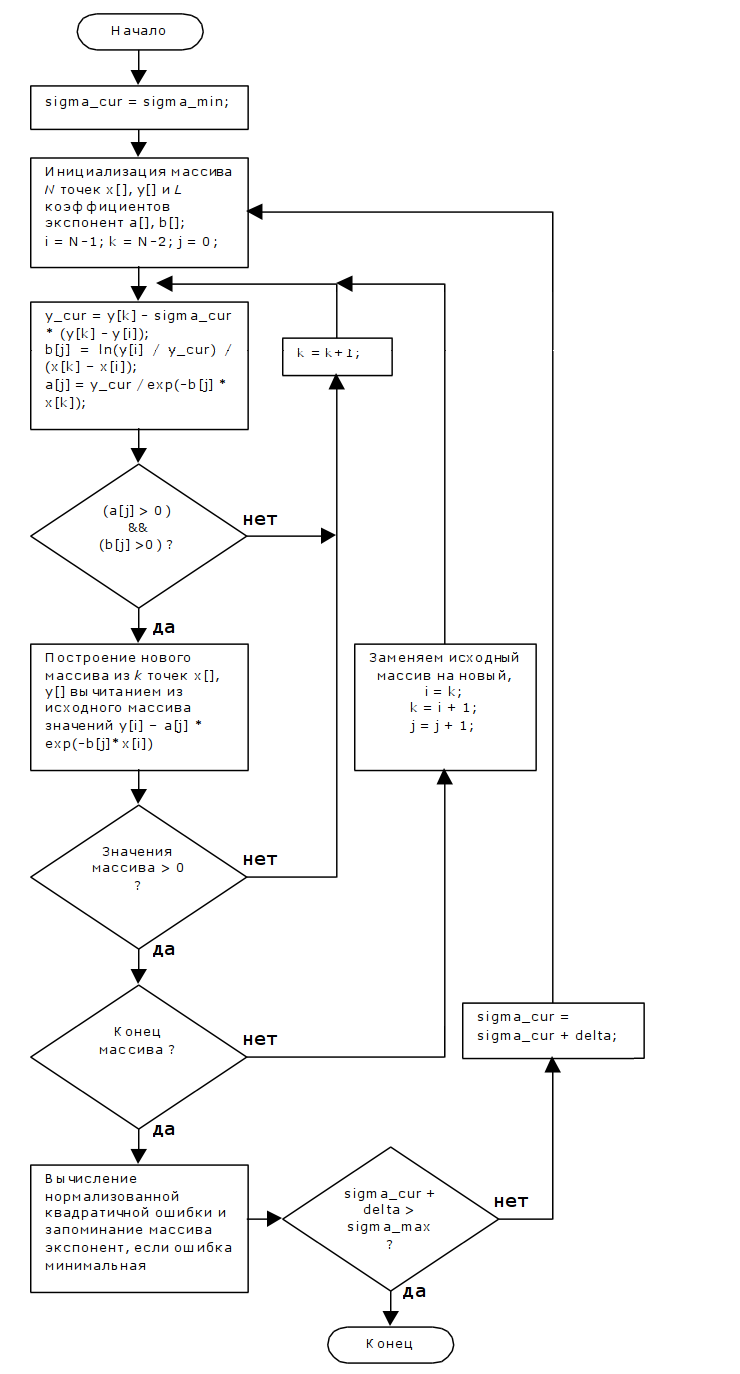
\includegraphics [scale=0.67] {greedy_schema}
  \caption{Блок-схема жадного алгоритма} 
  \label{img:greedy_schema} 

\end{figure}
%todo Рис. 1

\subsection{Алгоритм Левенберга-Марквардта}\label{subsect2_4_4}

Алгоритм Левенберга-Марквардта используется для оптимизации функций вида:

\begin{equation}
\tag{\ref{eq:square_minimum}}
F(x) = \frac{1}{2} \displaystyle \sum_{i=1}^N \phi_i(x)^2,
\end{equation}
при этом используется алгоритм градиентного спуска:

\begin{enumerate}
 \item Задается начальное приближение $\vec{x_0}$ и точность рассчета $\epsilon$;
 \item Рассчитывается $ \vec{x_{i+1}} =  \vec{x_{i}} - \gamma \nabla F(\vec{x_{i}}) $;
 \item Проверяются условия $\left| \vec{x_{i+1}} - \vec{x_{i}} \right| > \epsilon, \left| F(\vec{x_{i+1}}) - F(\vec{x_{i}}) \right| > \epsilon $ если условия верны, то $i = i + 1$ 
 и выполняется шаг 2, иначе итоговый вектор $ \vec{x} = \vec{x_{i+1}} $.
\end{enumerate}
%особый вид матрицы Гессе.
Обозначим через $J(x) m \times n$-матрицу Якоби для $f(x)$ и пусть $G_i(x)$ --- 
матрица Гессе для $f_i(x)$. Тогда выражения для градиента $g(x)$ и матрицы Гессе $G(x)$ функции
(\ref{eq:square_minimum}) будут выглядеть следующим образом:
\begin{equation}
\begin{split}
 g(x) &= J(x)^T f(x); \\
 G(x) &= J(x)^T J(x) + \displaystyle \sum_{i=1}^M f_i(x) G_i(x).
\end{split}
 \label{eq:levenberg_gesse}
\end{equation}
% Отсюда видно, что элементы $G(x)$  образованы комбинациями первых и вторых 
%производных функций $f_i$
%todo ньютоновская система.
Обозначим через $x_k$ текущую оценку решения задачи минимизации функции (\ref{eq:square_minimum}),
тогда ньютоновская система в силу (\ref{eq:levenberg_gesse}) примет вид:
\begin{equation}
 \left(J^T_k J_k + Q_k\right) p_k = -J^T_k f_k.
\end{equation}
Её решением будет вектор $p_N$ --- ньютоновское направление. В случае алгоритма Ньютона-Гаусса, оно аппроксимируется  решением системы 
\begin{equation}
 (J^T_k J_k ) p_k = -J^T_k f_k.
\end{equation}
Данная задача разрешима и включает только первые производные от $f$.

В алгоритме Левенберга-Марквардта направление поиска 
определяется, как решение системы уравнений вида:

\begin{equation}
 (J^T_k J_k + \lambda_k I) p_k = -J^T_k f_k,
\end{equation}
$\lambda_k$ - некоторое неотрицательное число. В этом методе шаг вдоль $p_k$ всегда 
полагается единичным, т.е. очередная точка $x_{k+1} = x_k + p_k$. Монотонное убывание минимизируемой
функции достигается за счет подбора <<хороших>> значений $\lambda_k$. При $\lambda_k = 0$, направление будет 
направлением Гаусса-Ньютона, когда $\lambda_k \to \infty$ норма $p_k$ стремится к нулю, и вектор
$p_k$ в пределе становится параллельным антиградиенту. Неравенство $F (x_k + p_k) < F_k$ можно обеспечить
выбрав $\lambda_k$ достаточно большим. Однако при этом теряется информация о кривизне, и проявляются
недостатки метода градиентного спуска --- в места пологого наклона необходимо делать большие шаги, чем в случае
с крутым наклоном. Марквардт ввел модификацию в алгоритм Левенберга, учитывающую кривизну

\begin{equation}
 \left(J^T_k J_k + \lambda_k diag \lbrace J^T(\vec{x_k}) J(\vec{x_k} \rbrace \right) p_k = -J^T_k f_k.
\end{equation}

Затем с вектором $p_N$ проводится процедура градиентного спуска.

%todo Модифицированный алгоритм Левенберга-Марквардта

\subsection{Тестирование алгоритмов}

Исследованные алгоритмы были реализованы на языках octave (Левенберг-Марквардт, Прони), Python (Численный перебор параметров),
 LabVIEW (модификация жадного алгоритма). Алгоритмы были протестированы на 68 сериях измерений по 10 измерений в каждой серии.
 34 серии были сгенерированы с помощью метода Монте-Карло, 34 с помощью генерации целевых функций. 

Результаты тестирования представлены на графике (\ref{img:generated_exp_data})

\begin{figure} [h]
  \center
  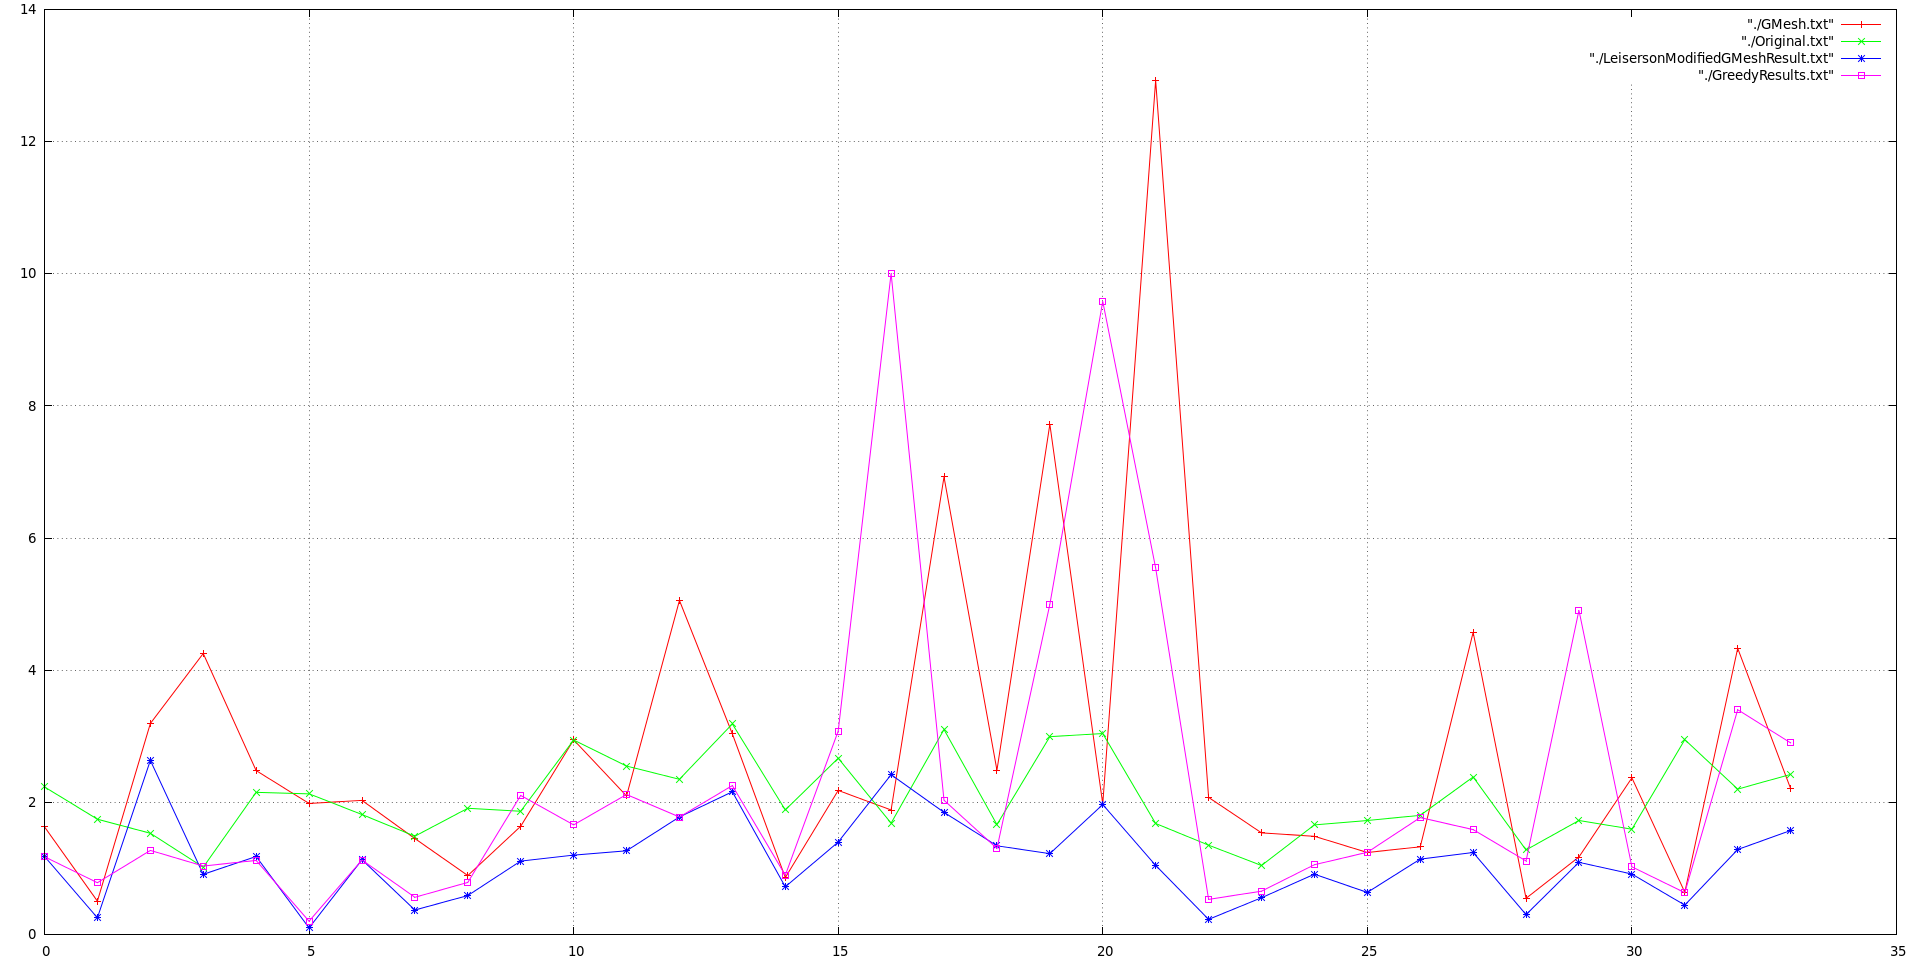
\includegraphics [scale=0.35] {generated_exp_data}
  \caption{Результаты тестирования на алгоритмах} 
  \label{img:generated_exp_data} 

\end{figure}

На данном графике по оси абсцисс отображены номера серий измерений (от 0 до 33), по оси ординат --- значения ошибок на данных
 при полученных параметрах экспонент.

На уровне около 2\% находится график оригинальных экспонент без шума. В среднем, алгоритм Левенберга-Марквардта 
получает результат лучший, чем оригинальные экспоненты, однако на ряде точек перебор параметров и модификация
 жадного алгоритма показывают меньшую погрешность. По этой причине был предложен и реализован комбинированный алгоритм.


\subsection{Комбинированный алгоритм}

Предложенный комбинированный алгоритм состоит из двух частей: 

В первой части вычисляются начальные оценки $a_i, b_i$ параметров экспонент с помощью численного перебора и модификации жадного алгоритма. 
Далее вычисленные значения передаются в качестве первичных оценок в алгоритм Левенберга-Марквардта
 и модифицированный алгоритм Левенберга-Марквардта. Затем, из первичных оценок и результатов работы алгоритмов
 выбираются параметры экспонент, на которых норма (\ref{eq:zuybin_petuhov}) принимает минимальное значение,
 эти параметры возвращаются в качестве результата работы алгоритма  (\ref{img:combined_algorithm}).
\begin{figure} [h]
  \center
  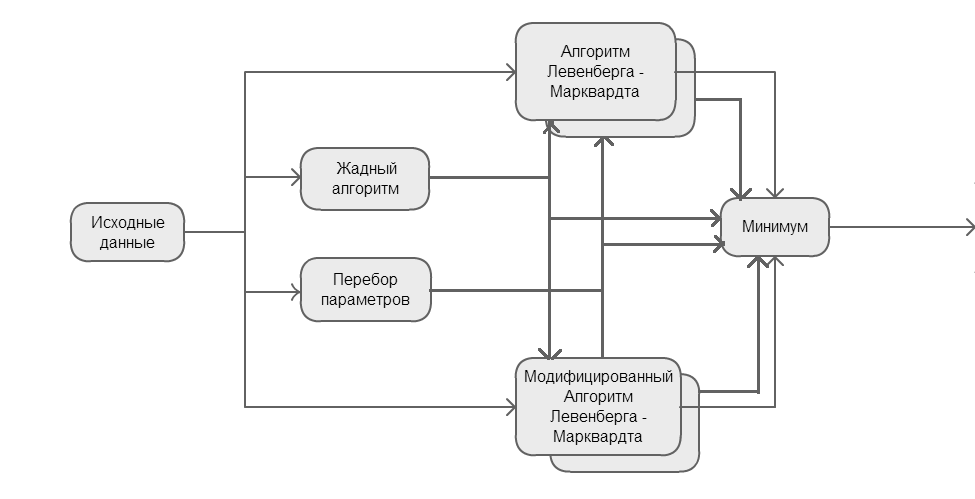
\includegraphics [scale=0.65] {combined_algorithm}
  \caption{Схема комбинированного алгоритма} 
  \label{img:combined_algorithm} 

\end{figure}


\section{Архитектура системы автоматизации обработки данных}\label{subsect2_5}

Рабочее место оператора состоит из <>. Оператор получает файл с тарировочными кривыми, затем АРМ оператора считает, рисует график, проводится измерение
\clearpage
